%%%%%%%%%%%%%%%%%%%%%%%%%%%%%%%%%%%%%%%%%%%%%%%%%%%%%%%%%%%%%%%%%%%%%%
% LaTeX Example: Project Report
%
% Source: http://www.howtotex.com
%
% Feel free to distribute this example, but please keep the referral
% to howtotex.com
% Date: March 2011 
% 
%%%%%%%%%%%%%%%%%%%%%%%%%%%%%%%%%%%%%%%%%%%%%%%%%%%%%%%%%%%%%%%%%%%%%%
% How to use writeLaTeX: 
%
% You edit the source code here on the left, and the preview on the
% right shows you the result within a few seconds.
%
% Bookmark this page and share the URL with your co-authors. They can
% edit at the same time!
%
% You can upload figures, bibliographies, custom classes and
% styles using the files menu.
%
% If you're new to LaTeX, the wikibook is a great place to start:
% http://en.wikibooks.org/wiki/LaTeX
%
%%%%%%%%%%%%%%%%%%%%%%%%%%%%%%%%%%%%%%%%%%%%%%%%%%%%%%%%%%%%%%%%%%%%%%
% Edit the title below to update the display in My Documents
%\title{Project Report}
%
%%% Preamble
\documentclass[paper=a4, fontsize=11pt]{scrartcl}
\usepackage[T1]{fontenc}
\usepackage{fourier}

\usepackage[english]{babel}															% English language/hyphenation
\usepackage[protrusion=true,expansion=true]{microtype}	
\usepackage{amsmath,amsfonts,amsthm} % Math packages
\usepackage[pdftex]{graphicx}	
\usepackage{url}

\usepackage{color}
\usepackage{multicol}
\setlength{\columnsep}{1cm}
\usepackage{graphicx}
\graphicspath{{images/}}
\setlength\parindent{0pt}
\usepackage{array}
\usepackage{float}

%%% Custom sectioning
\usepackage{sectsty}
\allsectionsfont{\centering \normalfont\scshape}


%%% Custom headers/footers (fancyhdr package)
\usepackage{fancyhdr}
\pagestyle{fancyplain}
\fancyhead{}											% No page header
\fancyfoot[L]{}											% Empty 
\fancyfoot[C]{}											% Empty
\fancyfoot[R]{\thepage}									% Pagenumbering
\renewcommand{\headrulewidth}{0pt}			% Remove header underlines
\renewcommand{\footrulewidth}{0pt}				% Remove footer underlines
\setlength{\headheight}{13.6pt}


%%% Equation and float numbering
\numberwithin{equation}{section}		% Equationnumbering: section.eq#
\numberwithin{figure}{section}			% Figurenumbering: section.fig#
\numberwithin{table}{section}				% Tablenumbering: section.tab#


%%% Maketitle metadata
\newcommand{\horrule}[1]{\rule{\linewidth}{#1}} 	% Horizontal rule
\definecolor{darkgreen}{RGB}{0,153,76}

\title{
		\vspace{1in} 	
		\usefont{OT1}{bch}{b}{n}
		\normalfont \normalsize \textsc{Iowa State University} \\ [25pt]
		{\color{darkgreen}\horrule{1pt} \\[0.5cm]}
		\huge CAndroid \\
		{\color{darkgreen}\horrule{1pt} \\[0.5cm]}
		\large Android Bridge for Off-Highway Vehicles
		\vspace{1.25in}
}

\author{
		\normalfont 								\normalsize
		{\color{darkgreen} Group Dec 14-02}\\ \normalsize
        Alec Johanson\\[-3pt]		\normalsize
        John Shelley\\[-3pt]		\normalsize
        Ahmmad Shelley\\[-3pt]		\normalsize
		\\ \normalsize
		{\color{darkgreen} Client}\\ \normalsize
		Vermeer \\ \normalsize
		\\ \normalsize
		{\color{darkgreen} Advisors}\\ \normalsize
		Arun Somani \\ \normalsize
		Koray Celik \\ \normalsize
}
\date{}

%%% Begin document
\begin{document}
\maketitle
\pagebreak
\tableofcontents
\pagebreak
\section{Problem}
Modern off-highway/agricultural systems use outdoor rated LCD displays to implement user interfaces. These current solutions are either too expensive, or put users at risk being an unsafe distance from the machines. Vermeer wishes to replace these expensive display systems with a more inexpensive solution as well as provide a more flexible development environment. A J1939 CAN system is used on most Vermeer systems, but would like to be expandable to other protocols. Vermeer has expressed their wish of emphasizing research and development with solutions utilizing Android systems due to their prior experience with this technology. \\

Vermeer currently uses a CAN bus to communicate data from a machine, such as a baler, to a VT (Virtual Terminal) in the cab of the tractor that is towing it. These VTs are wired, and proprietary. This makes them expensive and exposes the CAN bus to the harsh Agricultural environment. Replacing the Virtual Terminal with an Android device has the potential to greatly reduce cost. While making the connection to the Android device wireless can help assist in erosion prevention of the system. \\

\subsection{System Requirements}
\vspace{10pt}
\begin{tabular}{c | c}
	\textbf{Functional} & \textbf{Non-Functional} \\ [2ex]
	Stream > 10\%  CAN bus load at 250Kbps throughput & User friendly for the Android operator \\ [1ex]
	Withstand outdoor environment & Extensible to other CAN protocols \\ [1ex]
	Withstand high vibration environment & \\ [1ex]
	less than \$300 unit cost & \\ [1ex]
\end{tabular}

\subsection{Functional Decomposition}
The main communication pertaining to our project is between a VT (virtual terminal) and a controller on the unit (in our target case a 605 baler). The controller communicates to the VT through a CAN bus starting with a series of hand shakes, setting up the initial UI. Then during normal operation, the controller reads data from point to point connections with sensors. The controller analyzes the data and sends UI update information through the CAN bus. This connection between the controller and the VT will now be wireless utilizing Android instead of a proprietary VT system. \\

\pagebreak
\section{Solution}
\subsection{Solution Space}
For the solution we needed a way to receive a CAN signal at a fairly rapid rate. We also needed at way to communicate with the Android device wirelessly. Third, we needed a way to translate the CAN signal to a format understandable by the Android Device. These could all be done with a single module, or seperate modules for each task. A balance needs to be taken into consideration when comparing module selection to minimize complexity while maximizing modularity.  \\

\subsection{Chosen Solution}
The solution chosen was to use a PIC32MX795 microcontroller to receive CAN data from the controller on the operating machine. The PIC32 communicates with a WRTnode module that runs a web socket for wireless communication with the Android device replacing the Virtual Terminal.\\

\subsection{System Analysis}

\textbf{Controller} \\
The controller obtains information from outside diagnostic tools on the machine. The controller then analyzes this information to determine what updates are needed for the VT. Another function of the controller is to send commands to these peripherals. \\

\textbf{RF Bridge} \\
The RF Bridge is what receives information from the Controller through the CAN Bus. This will then distribute the information over a wifi signal. Since a cloud connection is less feasible due to operating conditions,  an AdHoc similar network approach will take place. \\

Our solution for the RF Bridge was to use a WRTnode, running a version of embedded linux to act as a server for the Android device. The WRTnode can not directly receive a CAN signal so a PIC32 microprocessor translates the CAN data to UART for the WRTnode to receive. \\

\textbf{Android Device} \\
Input from the RF bridge is then received by the Android device. Data from the RF bridge is received as JSON and parsed by the device into VT elements. The Android device then outputs the parsed data to the User Interface showing the current machine state. \\

 \pagebreak
 Details of the modules are expanded upon in the following sections. Shown in Figure 2.1, shows a high level block diagram of our solution.  \\
 \begin{figure}[h]
	 \center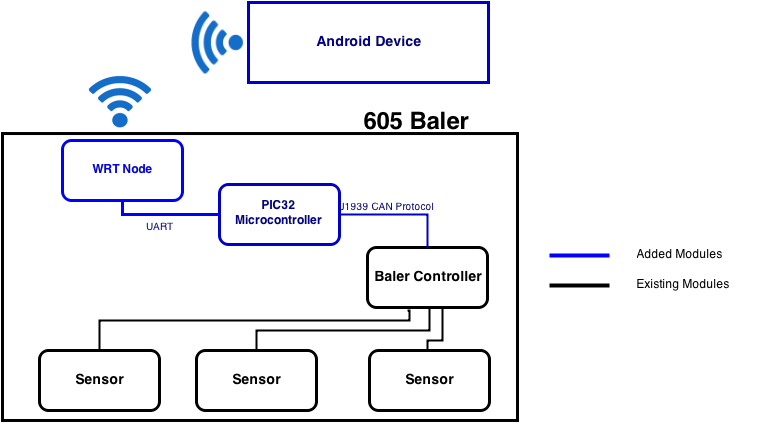
\includegraphics[scale=0.6]{rev4.png}
 \caption{High-Level Block Diagram of Solution}
 \end{figure}

\subsection{Hardware Description}
\textbf{PIC32 Microcontroller}  \\
The most important requirement of the microcontroller we selected was that it needed to be able to receive and interpret CAN signals efficiently. The PIC32 microcontroller has multiple families, of which, all PIC32MX5xx, PIC32MX6xxx, and PIC327xxx microcontrollers have CAN modules. We selected the PIC32MX795 due to it's increased memory and computing capacity. We wanted to select a microcontroller that was overpowered rather than underpowered due to the time it takes to deliver the microcontrollers. The PIC32MX795 offers 512KB of program memory, 128KB of ram, UART and SPI modules, as well as the CAN modules stated before. This fulfills all specs required of the microcontroller. \\

The microcontroller is responsible for receiving data from the CAN bus and converting that data to UART so the WRT node can understand it. The data sent over the CAN bus will first be a file called an IOP file. This file gives the initial state of the display for the VT/Android Device. After the IOP file is sent, all subsequent data transfers are updates to the display.  \\

The microcontroller is also responsible for communication in the opposite direction. While the machine is running, the Virtual Terminal can send commands to the machine through various buttons on the screen, such as "Dump Bale". The microcontroller receives these commands via UART from the WRT node and sends a corresponding message on the CAN bus to the controller on the baler. \\

\textbf{WRTnode} \\
We didn't start using the WRTnode until late in the development cycle. After long chains of communication, the need for the WRTnode arose due to the IOP parser being written in python. The WRTnode runs a flavor of embedded linux called OpenWRT, hence the name of the device. The device was limited to the amount of storage it was able to hold , so we ended up mounting a USB drive with approximately 16 GB of storage. This allowed for a larger set of source code for the python program. \\

The Node housed our WebSocket server, written in python. Unlike most RESTful API based web servers, a WebSocket server allows for continuous communication between a server and its clients through the use of sockets. A client, in our case an Android Tablet, can issue a command to the server. If the command is the "Start" command that the server was expecting then they establish a handshake. The two can now freely talk to each other. The benefit of this allows the server to notify the client of an update, without the client needing unnecessarily refresh, like most ajax environments. \\

The WRTnode is beneficail over other design possibilities because of its ease of use, mobility, cost. The cost of the two XBEE wifi modules was more, and the Node was much easier to work in a language and environment that we were well familiar with. However, in a highly variable environment that most tractors and balers are positioned in, Vermeer may choose to write a 'C' program on the PIC and communicate directly with the XBEE's if it is faster and more efficient than the python program. \\

\textbf{Nexus 7} \\
The Nexus 7 is targeted in this project but not required. Almost an Android tablet will be compatibale depending on the consumers needs and wants. \\

The Nexus 7 is an Android tablet. It is 7 inches, which is about 1 inch smaller than most tablets on the market currently (such as those from Apple, Samsung, and LG). First released in 2012, and updated in 2013, the Nexus 7 is still considered to be of high quality in both hardware and software. Compared to the other tablets on the market the Nexus is the most cost effective choice. If you needed something of higher quality you will have to spend significantly more than the approximate price of \$180.00. These all contributed to our choice and why we went with the Nexus 7. However, with the current release of the Nexus 9, the 7's are no longer being sold on Google's website. Thankfully the Android OS doesn't constrain us to one specific device. \\

The Client software is a pure translation of the Virtual Terminal that most of the current tractors use in their cabs. It is a very low level software system that was originally designed for harsh environments. Basic software elements include: input texts, output texts, graphical objects, meters, bar graphs, buttons, and macros that can be associated with any of the aforementioned items. The Android SDK, has a wide array of resources used to convert and translate any of the given Virtual Terminal predefined Software Components into native Android code. In order to do so, we set off first documenting our approach to translating the given components from the Virtual Terminal systems to Android Views. This information can be found in the supplemental document "Android UI Guidelines".  \\

\textbf{XBee WiFi Modules (XB2B-WFST-001)} \\
The Xbee WiFi modules were not used in the final design. They were originally selected to make an ad-hoc connection between the microcontroller and the Android device. We selected this particular model because of the ability to add any size antenna. This would have helped in testing to see what the minimum size antenna for a certain distance would require. Even though the XBees weren't used in the final design. They proved to be a viable secondary option for Vermeer. They also aided in debugging connections on the final design, since we had proven earlier that the connections worked with them. Knowing these worked allowed us to run the WRTnode in sync with the XBees, verifying the incoming data was correct on the CAN bus, thus, eliminating a debugging step when a problem arises. \\

\pagebreak
\subsection{PCB Design}
 \begin{figure}[ht]
	 \center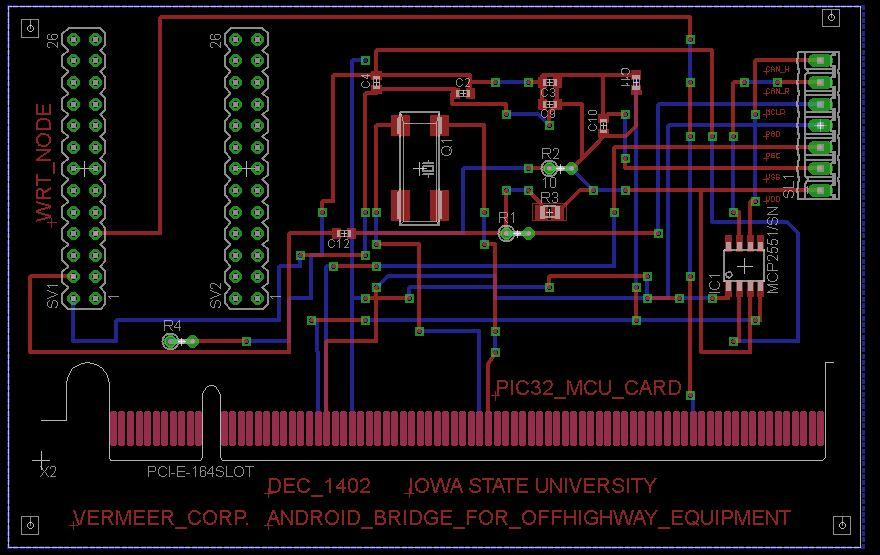
\includegraphics[scale=0.4]{PCB.jpg}
 \caption{Printable Circuit Board Design for Rev. 4}
 \end{figure}

 \vspace{30pt}

 \subsection{Unit Cost}
 \vspace{10pt}
 \begin{center}
 \begin{tabular}{l c c c}
	\hline\\
	 \textbf{Unit} & \textbf{Qty.} & \textbf{Unit Price (\$)} & \textbf{Total Price (\$)} \\ [1ex]
	 PIC32MX795F512L & 1 & 9.87 & 9.87 \\ [1ex]
	 WRTnode & 1 & 25.00 & 25.00 \\ [1ex]
	 MCP2551 & 1 & 1.22 & 1.22 \\ [1ex]
	 Nexus 7 & 1 & 180 & 180 \\ [1ex]
	 Misc. (Capacitors, etc.) & & <10 & <10 \\ [1ex] \cline{4-4}
	 \textbf{Total}&&& \textbf{~226.09} \\ [1ex]
	\hline
\end{tabular}
\end{center}
 

 \pagebreak
 \section{Operation Manual}
 \subsection{Microcontroller} 
 The microcontroller works as soon as it is turned on if the program has already been loaded. If the program is not loaded, attach the microcontroller to the devboard and connect with the PC. Open the project containing the correct code and simply press the "Build and Program" button in the IDE. This will open microProg and automatically begin programming the microcontroller. The development board will have a blue flashing light while the board is programming. When the programming is done, the blue light will cease flashing, and a red LED will blink on the main LED grid as a status that the program is running. \\
 \subsection{WRTnode}
 The WRTnode must have a power source. It came included with a split USB cable for mounting USB drives, and a second male connector to charge from a laptop. It also has the capabilities for being powered through a 3.3 Volt pin. Once turned on, in order to access the WRTnode's shell, you have to connect to its broadcasted SSID signal. Once connected, you can open a terminal and ssh into the node. \\

 Once inside the shell of the node, you can do all sorts of things. For the scope of this project, run the ./mountUSB.sh script. This mounts the USB storing our server code. From there cd to the USB mounted at /mnt/shares. Inside the USB's main folder should be another script called ./update.sh. This removes and old code and pulls down any new code from github. The reason for the USB was limited storage space on the WRTnode, and our Python server contained 4 libraries, one of which was hefty in size because of the asynchronous networking code. Another tool we use is virtual environments. This allows us to install any libraries to a separate folder so our main python install doesn't get crowded, and it is specific to this project only. If you are unable to see a "(vermeer)" before the beginning of every line in the console, then you are not correctly inside the virtual environment. In order to do so, type source vermeer/bin/activate. You should now be ready to operate the server.\\ 
 In order to run the code, make sure you are in the folder called vermeer-backend-master. Once inside execute python vermeer/backend/server\_asyncio.py. You can also execute this with a -debug flag for a more verbose output usefull for testing purposes. The server will now wait until it gets a "Start" command from the CAN and PIC controller. Once started, the server will always be listening on 192.168.1.1. However, you are only allowed to talk to it if you are connected to its broadcasted SSID as well, which you are allowed to make password protected. As soon as a client connects to it, it then goes through steps to determine whether to initialize the Virtual Terminal, or to update an existing one. It then parses the .iop file for specific components and constructs a json blob to send back the client to display the terminal. \\
 
 \begin{samepage}
 Any updates sent from the CAN through the PIC to the server, will be sent out to all connected clients. The clients must update their displays and respond with a success or error message. \\
 \end{samepage}
 
 \begin{samepage}
 If any client disconnects at any time, whether on purpose or accident, the server will know recognize this and terminate the connection on its end as well, this automatic termination frees up space and memory. \\
 \end{samepage}

 \subsection{Android Device} 
 To operate the Android tablet we must first have turned on with a charge. Once the device is on, we have a couple of choices on how we plan to install the application. We can default to putting the application on the Google Play Store, which allows anybody in the given locales to download it. We can also use Google Community groups to allow only a select few from seeing it in the play store, but this is a hassle for any user needing to download it with short notice. Another option is through third party distributes such as TestFlight, which allows people to sign up via email to receive a download of the app. And finally we can simply install the .apk ourselves through manual transfer, whether by email or a download link from a website. Since there is little security risk, putting the application directly on the Google Play Store would be recommended for ease of access to customers. \\

 As soon as the app is installed, open the app by clicking on it from the launcher or app drawer. Once signed in, the user is given one option, to start the Terminal. The app then runs a set of background tasks to pull down information from our WebSocket server. This will include all of the components from the .iop file such as output texts, input texts, pictures, graphics, charts, and commands. The Android app then builds all of these using gson to convert the json blobs. Based on what is sent from the server, the views are constructed either dynamically or manually. \\

 Once the UI is constructed the user now has free reign over the tablet in regards to any predefined program issued from the CAN and .iop. This includes clicking any buttons, inputting any information, and performing tasks. The Android application is always listening to the WebSocket server through an open port that was established during the handshake procedure. This allows the server to update any ui components at any time of the duration of the app as well. \\

 Once a user is done using the app, they can safely turn off the terminal by selecting the disconnect button at the top. This is recommended over simply turning off the screen or pressing either the home or back button, because it allows the server to know that we wanted to safely disconnect and that it wasn't an error that caused the disconnect. \\

 \subsection{Summary} 
 Make sure the WRTnode is turned on and functional. Currently, it is required to ssh into the server to start it manually given the steps above. In the future we would plan to create a startup script that runs on boot, that mounts our USB drive, runs the update script, and runs ther server. After the WRTnode is turned on and functionally, it will be waiting for the PIC to send it a  message. As soon as any CAN Controller is turned on (like our 605 Baler model) it should transmit a signal through its CAN interface to the PIC. The PIC will then send a "Start" signal to the server to turn let the server on the WRTnode know that the CAN and any Controllers are in use. The Android tablet can now connect by following the above steps and clicking the "Start" button on the device. \\

 \pagebreak
\section{Testing}
\subsection{CAN-UART Connection}
The CAN bus was tested using Vector VN1630 hardware with varying CAN messages that were  controlled by CANalyzer software. The CAN-UART connection was first tested by sending the CAN messages to the UART connection that was connected to 	WiFi to a computer. The received messages then, was verified to be the same as the send messages. \\

\subsection{Endurance Testing}
The CAN-UART connection was run in excess of 5 hours to test the endurace of the system. Endurance testing was done to mainly make sure the program didn't crash. If the program did crash, it would likely have been due to a memory leak. During the endurance testing, the inputs and outputs through the system were verified to be equivalent. \\

\subsection{Interference Testing}
Interference testing was conducted utilizing the Vector module. The vector module mimicked additional modules sending traffic on the CAN bus. The program was able to detect correct data and filter unwanted data. \\

\pagebreak
\section{Design Revisions}
\subsection{Design Revision v1} 
 \begin{figure}[H]
	 \center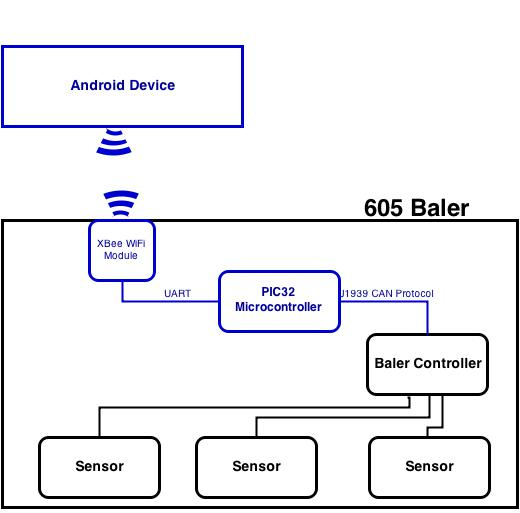
\includegraphics[scale=0.4]{rev1.jpg}
 \caption{Block diagram for design revision 1}
 \end{figure}
Our original design featured a single XBee WiFi module. XBee WiFi modules offer either a UART or SPI interface to transfer data up to 6Mbps. We soon found early on that the XBee is easily connected to the Android device but only through the cloud service. In our project we did not have access to the cloud with the current design. This impediment was resolved in revision 2.\\

\subsection{Design Revision v2} 
 \begin{figure}[H]
	 \center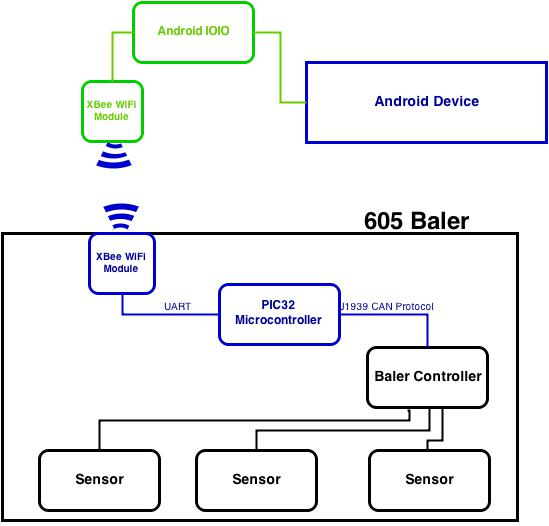
\includegraphics[scale=0.4]{rev2.jpg}
 \caption{Block diagram for design revision 2}
 \end{figure}
In design revision 2, we solved the problem of not being able to connect to the cloud by adding another XBee. XBees have the ability to connect and communicate with each other without the need for a cloud service. We also needed a way for this additional XBee module to communicate with the Android device. This was accomplished using an Android IOIO (pronounced YO-YO). The Android IOIO can connect to the Android Device using a USB plug or via bluetooth. The Android IOIO can then act as a pipe for the UART data from the XBee to the Android device. \\

This revision has the possibility to be suitable in use cases other than the 605 baler. The baler is more specific in our case because of the VT. In some scenarios, it has been expressed that Vermeer may wish to simply "dump information" to an Android device. If simple data needs to be sent and there needs to be little parsing, that is, parsing that can feasibly be  done in a 'C' program directly on the microcontroller, this is a possible solution. With this solution, the data can then be later transferred to a computer to execute more rigourus parsing and analyzation. In this case, the Android device may simply act as a vessel to carry the data from the machine to a computer. The advantage of the XBee modules is the ability to network with multiple XBees. This way, multiple devices can receive the data at the same time. With the model of XBees that we selected, Vermeer has the ability to choose which antenna's to add to the XBees based on the range and price required. \\

\subsection{Design Revision v3} 
 \begin{figure}[H]
	 \center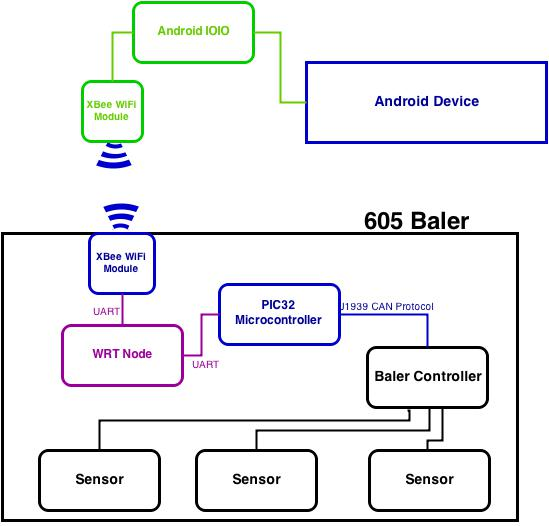
\includegraphics[scale=0.4]{rev3.jpg}
 \caption{Block diagram for design revision 3}
 \end{figure}
Up until this revision, we had been communicating with Vermeer to figure out how we would parse the IOP file in the same manner that the VT does. We decided that we wanted to do as much parsing of this data before transferring over WiFi to save processing power on the Android device thus reducing battery consumption and improving performance. Vermeer had an early stage parser that was written in python. With the time constraints of the project we decided it would be more practical to attempt to implement and finish their partial parser, instead of creating a similar program in C. Using this program meant we could not use the PIC32 to handle the parsing of the IOP file. To run python we chose to use the WRTnode. The WRT node then received the IOP file from the PIC32, parsed it, and sent the data to the XBee modules. \\

\subsection{Design Revision v4} 
 \begin{figure}[H]
	 \center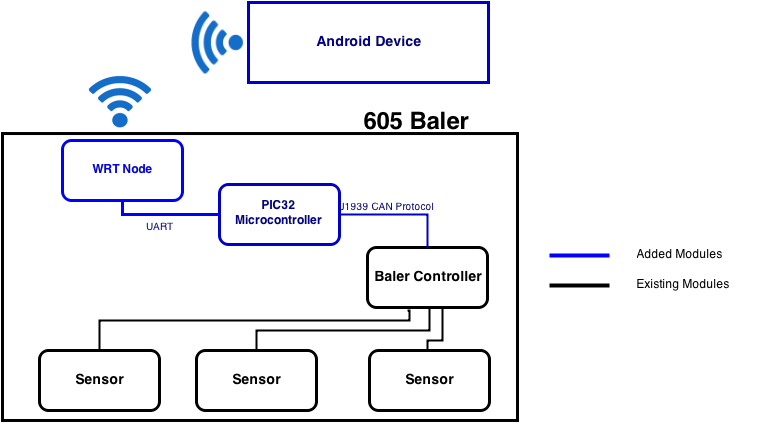
\includegraphics[scale=0.4]{rev4.png}
 \caption{Block diagram for design revision 4}
 \end{figure}
Design Revision 4 changes were made from Design Revision 3 because the WRTnode is able to directly communicate with the Android device. Removing the XBee modules removes 3 modules, greatly reducing complexity and cost. The USB port is available now that the Android IOIO does not need to connect to communicate with the Android device.\\

\pagebreak
\section{Tools}
\subsection{Development Tools}
\textbf{Vector}\\
Vector is very useful tool for debugging with CAN buses. We used the vector VN1630. With the Vector hardware (along with CANalyzer software) traffic can be read on the CAN bus, as well as transmitted. Vector is capable of mocking two modules on the bus. This allowed us to easily conduct interference testing without additional tools. Although in early debugging we diagnosed problems with an oscilloscope, the Vector saved us days, even weeks, of debugging and manually reading/translating CAN signals.\\

\textbf{Development Board}\\
The development board used for this project was an LV-32MX v6 PIC32 Development System. We chose to use this mainly for the purpose of programming. Programming the PIC manually proved to have finicky voltage regulation and the chip burned. The opportunity cost of solving the programming problem was too great, and the use of a development board was chosen. This system is one generation out of date, but still available. Therefore, when ordering chips with breakout boards, it is important to match with development board, as the pin layout differs greatly.\\

\textbf{MicroC/MicroProg}\\
MicroC is the IDE/Compiler used for the PIC32 microcontrollers. Like many embedded system IDE's the usability could be greatly improved. However, the program succeeded in it's intended purpose.\\
MicroProg is the program for uploading a new program to the micro-controller. Again, the usability could be slightly upgraded, but successfully accomplishes its goals.\\

\textbf{XCTU}\\
XCTU is an extremely helpful tool in debugging and testing XBee modules. It is also a simple way to reconfigure settings on the XBee modules such as the baud rate, SSID, and network type. XCTU is the most usable program that we used. Including a very intuitive user interface for receiving and sending data via the XBee modules.\\

\subsection{Organizational Tools}
\textbf{Slack (slack.com)}\\
Slack is a team communication platform. Much like email, or any other chat based platform, however it allows for some heavy customizations and multiple integrations. Any github commit, trello change, or google hangout, will show up in Slack. Slack allows for multiple channels, so a single feed isn't constantly getting clogged up as well. We used channels like \#Software, \#Hardware, and \#General.\\

\textbf{Trello (trello.com)}\\
Trello is free ticket management system. Trello allows you to make tickets with labels on them, we had labels such as "Hardware", "Software", "Documentation", etc. Trello also allows for customized lists, we had a simple set of lists "TODO", "In Progress", and "Done". Some helpful additional lists could be "In test" and "Ready for testing".  Users can also be assigned to tickets (or multiple users) and comments can be made. A useful feature different than some other ticket management systems is the ability to add checklists inside of a single ticket, as opposed to making multiple tickets. Trello is comparable to Atlassian JIRA for those who are familiar.\\

\textbf{Github (github.com)}\\
Github is a popular version control system. We used this for code on all of the modules. This proved to be very useful comparing code between revisions that worked and revisions that didn't. Github has also been useful for reviewing other member's code changes through pull requests and Github's diff tool.\\

\pagebreak
\section{Setbacks/Challenges} 
The biggest setback we had during the project was communication. There were multiple times when lack of quality communication (sometimes out of our control) cost us weeks of development time. At the beginning of the project it took us longer than anticipated to fully understand the scope of our project. A day trip to Vermeer's corporate headquarters meeting with our Vermeer contact and others helped alleviate this initial confusion. After the trip to Vermeer, designing solutions emerged at a more rapid pace. Another instance where lack of quality communication stalled progress was on the software side. We knew that we would receive and IOP file and needed to parse it. Learning how to parse this IOP file proved to be much more difficult than anticipated, and many meetings with the incorrect people, pointing us to the "correct" people impeded software development greatly. \\

Another setback that we had early on in development was programming the microcontroller. When attempting to program the microcontroller manually, the voltage was not regulated properly and burned the chip. To avoid this from happening again, when we ordered another chip, we also ordered a development board to assist in the programming process. This development board included a USB programmer to allieviate the voltage regulation problem. The development board also assited in debugging allowing messages to be displayed on an LCD display. \\

The third major setback that we had in development was getting the clocking to work so all the peripherals worked at the same time on the microcontroller. We had multiple sections working independently, however, during integration everything ceased to continue working. After strenuous debugging it was found that clocking, specifically, a phased-lock loop circuit was the culprit. After correcting this, development came along with few other setbacks. \\

A fourth challenge we faced was also related to communication. One of our group members needed to work remotely for approximately four months. This challenge was conquered with frequent video conferences. These video conferences consisted of progress updates, design decision discussions, as well as any other administrative needs. We also assigned tasks to that member that were not tightly coupled with the tasks that were currently being worked on on-site by the other group members. This allowed the remote group member to have greater autonomy thus reducing the need for immediate or frequent communication.

\pagebreak
\section{Reflection}
This project has taught us many things. With the hardware side, it was the first time any of us had created a hardware project from nothing. Previously, we were given instructions, skeletons, and hardware, then we simply built on top of that. A lot was gained from making the project with nothing to start. We learned about comparing and researching hardware modules. From this alone we learned about numerous technologies that we had never even heard of before. This also gave us experience in figuring out design specs so that it is possible to find which hardware will work well in a project.\\

In previous courses, we always used a normal breadboard to build a functioning circuit with different components of resistors, capacitors, LED's and operational amplifier. In this project, we used the Eagle PCB design software. It is the first time we had learned to build a PCB, as it is not taught in any specific courses. It is similar to a combination of pspice design software and layout design that we learned in two different courses. Attention to the details of the different pins and not to overlapping similar wires are important to avoid short-circuits or causing the circuit to behave in undesired ways.\\

On the software side a lot of new tools were used, and strange behaviors were observed. We knew the technology rather well. Android and python servers we were very familiar with. However, the way we used these tools were uncanny to say the least. With Android, layouts are predefined, and created during compile time that they might be viewed during runtime faster. Its just how the framework works. However to complete this project, we had to build the UI dynamically during runtime. We were worried this would affect runtimes and memory consumptions and management. On the server side, we tossed back and forth the idea of using full C code or python for the server. We ended up going with python because it was easier to implemented the type of server we wanted. However we learned interesting details when it came to parsing the .iop file such as how python packs bits into a struct. Our understanding of how an .iop file is created, and how it is read was challenged, but we now understand the overall process.\\

Even though it is well known and taught often, this project revealed even more so how important communication is. Slack greatly helped our internal communication channels. However, our communication channels with Vermeer lacked in comparison. This project showed us the importance of face-to-face communication. Our visit to Vermeer headquarters, and meeting in person at the Iowa State campus proved to be much more effective than phone calls, or even skype.\\

Our efficiency at reading data sheets has improved greatly over the course of the project. Before, in class, there was little need to look in data sheets, the needed data was often in the lab instructions. If we needed to look at a data sheet, where to look was usually pointed out to us. The autonomy of this project greatly improved our competency and efficiency in reading data sheets.\\

\pagebreak
\section{Future Iterations}
\subsection{Hardware}
A simple update to improve the system would be to upgrade the communications from UART to SPI. SPI requires an extra pin, but allows for faster data transmission. On the PIC microcontroller this allows for a theoretical \%600 increase in data speed. \\

Continued work needs to be done for manufacturing as well. The PCB should be printed and tested. A container for the unit should be designed as well to house the micro-controller and the WRTnode, without interfering with the wireless communication of the WRTnode. \\

\subsection{Software}
For the WRTnode, Server robustness could be improved. Currently waiting for data from the UART is a blocking process. The system would be more efficient and robust if a non-blocking thread listened for UART communication. \\

On the Android UI, more VT elements need to be recognizable to complete a fully functional application. The current parsing of VT elements can be used as a template.\\

Also, because of the dynamic structure we have created, there might be memory and time consumption issues. One way to resolve this, would be for the creator of the VT design (in this case Vermeer) to create an Android Layout file instead. They would then pass that file through the WRTNode, or potentially store it on the device, and just issue an id from the Node, which allows the android to call it up and inflate the layout. This allows for faster runtime loads, and for the android device to potentially store a numerous amount of layouts. The only drawback from this situation is the decoupling from the current VT ecosystem. The designers would have to design for two different systems, unless all of their consumers are using Android.
\end{document}
